\documentclass[11pt,onecolumn]{article}
\usepackage{amssymb, amsmath, amsthm,graphicx, paralist,algpseudocode,algorithm,cancel,url,color}
\usepackage{sectsty}
\usepackage{fancyvrb}
\usepackage{mathrsfs}
\usepackage{multirow}
\usepackage{hhline}
\usepackage{booktabs}
\usepackage[table]{xcolor}
\usepackage{tikz}
% \usepackage[framed,numbered,autolinebreaks,useliterate]{mcode}
\usepackage{listings}
\usepackage{enumitem}
\usepackage{cleveref}
\usepackage{tcolorbox}
\usepackage{mathtools}
\usepackage{pdfpages}
\graphicspath{ {./images/} }


\newcommand{\bvec}[1]{\mathbf{#1}}
\newcommand{\R}{\mathbb{R}}
\newcommand{\C}{\mathcal{C}}
\newcommand{\Rn}{\R^{n\times n}}
\newcommand{\Rmn}{\R^{m\times n}}
\newcommand{\Cn}{\C^{n\times n}}
\newcommand{\Cmn}{\C^{m\times n}}
\newcommand{\cO}{\mathcal{O}}
\newcommand{\ls}{\textsc{ls}}
\DeclareMathOperator{\Tr}{Tr}
\DeclareMathOperator{\trace}{trace}
\DeclareMathOperator{\diag}{diag}
\DeclareMathOperator*{\argmin}{arg\,min}
\DeclareMathOperator*{\argmax}{arg\,max}
\sectionfont{\Large\sc}
\subsectionfont{\sc}
\usepackage[margin=1 in]{geometry}
\DeclareMathOperator{\Tr}{Tr}

\DeclarePairedDelimiter{\abs}{\lvert}{\rvert}
\DeclarePairedDelimiter{\norm}{\lVert}{\rVert}
\DeclarePairedDelimiter{\innerproduct}{\langle}{\rangle}
\DeclarePairedDelimiter{\PAREN}{(}{)}
\DeclarePairedDelimiter{\BRACK}{[}{]}
\DeclarePairedDelimiter{\CURLY}{\{}{\}}

\newcommand{\bluebox}[1]{
  \begin{tcolorbox}[colback=blue!5!white,colframe=blue!75!black,boxrule=0.5pt,boxsep=0pt,left=6pt,right=16pt,top=4pt,bottom=4pt]
  #1
  \end{tcolorbox}   
}

\newcommand{\redbox}[1]{
  \begin{tcolorbox}[colback=red!5!white,colframe=red!75!black,boxrule=0.5pt,boxsep=0pt,left=6pt,right=16pt,top=4pt,bottom=4pt]
  #1
  \end{tcolorbox}
} 

\newcommand{\greenbox}[1]{
  \begin{tcolorbox}[colback=green!5!white,colframe=red!75!black,boxrule=0.5pt,boxsep=0pt,left=6pt,right=16pt,top=4pt,bottom=4pt]
  #1
  \end{tcolorbox}
} 

\begin{document}
\noindent
\textsc{\Large Numerical analysis: Project 1}\\
Instructor: Anil Damle\\
Due: March 10, 2025\\

By: Bodong Liu (bl576), Ryan Wu (rw645)
\bluebox{
\paragraph{Goal 1:}
Implement the Householder scheme for computing QR factorizations. Your QR factorization routine should take in a $n \times k$ matrix $B$ with $k\leq n$ and returns a $n\times k$ matrix $Q$ with orthonormal columns (or sufficient information to be able to apply it to a vector, e.g., the Householder vectors), and a $k\times k$ upper triangular matrix $R.$ Please demonstrate that your algorithm behaves as expected (this means both that you are getting a valid QR factorization as output and that it achieves the desired computational scaling). \textbf{Demonstrate that your implementation achieves the expected scaling and explain how you tested your implementation.}}

We perform the QR factorization using the Householder scheme, where given an input $B$ returns a set of orthonormal vectors $H_{vec}$ which can be used to reconstruct $Q$, and an upper triangular square matrix $R$ such that $QR=B$. The standard Householder scheme has an expected scaling of $O(mnl)$ where $l=\min \{m,n\}$, which in this case, $m\geq n$ for all inputs, thus there should be an expected scaling of $O(mn^2)$. 

At a high level, our algorithm (visible in code appendix), loops from $i=0...n$, and in each iteration of the loop, we find Householder reflection, which takes $O(m)$ operations, and perform the update $R[i:m,i:n] = R[i:m,i:n]-2v(v^\top R[i:m,i:n])$. This update consists of two vector-matrix multiplications, and then a matrix-matrix subtraction, which altogether requires $O(mn)$ operaions. Thus, each iteration has a time complexity of $O(mn)$, and it follows that the algorithm has an expected scaling of $O(mn^2)$. 

Next, we performed benchmarking to check the time complexity and scaling of our function. Below is the scaling on a log-log plot, specifically on tall-skinny matrices ($10n\times n$), which we see appears to scale around as expected at $O(mn^2)$.

$$
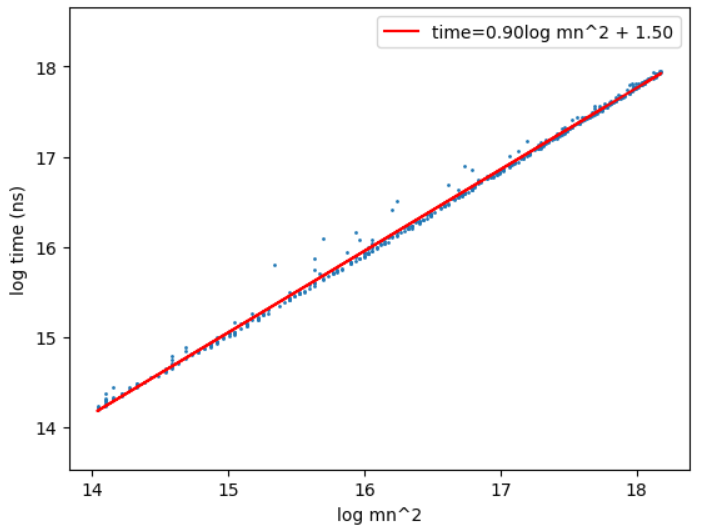
\includegraphics[scale=0.55]{./images/QRScaling.png}
$$
\newpage

We also benchmarked other cases: for square matrices, we have an expected time complexity of $O(n^3)$ because $m=n$. From the plot, it appears that there is indeed a cubic scaling factor. 
$$
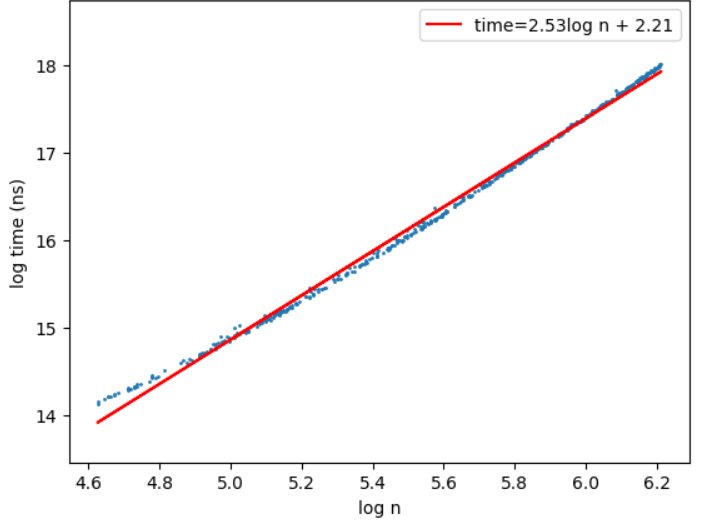
\includegraphics[scale=0.55]{./images/QRScaling_square.png}
$$

Below is the plot of our Householder algorithm on random $m\times n$ matrices, where $m\geq n$. Similarly, it is rather appropriately bounded by $O(mn^2)$.
$$
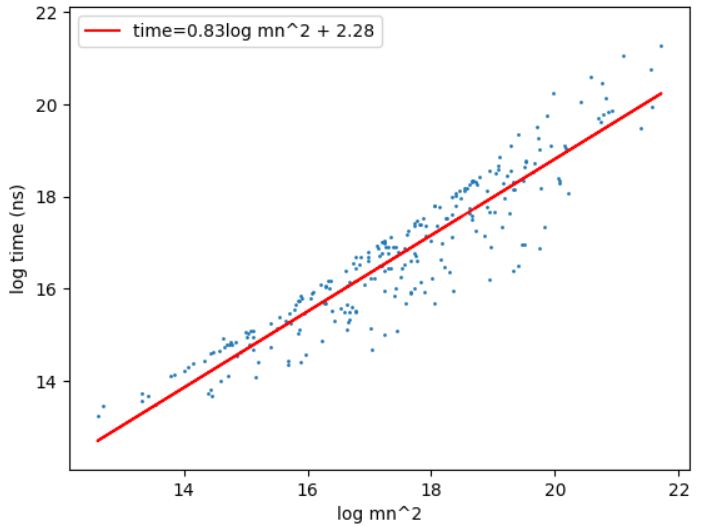
\includegraphics[scale=0.55]{./images/QRScaling_rectangular.png}
$$

To test our code, we created a script that generates 1000 random matrices $A$, where for each we explicitly compute $Q$ from the Householder vectors, then compare the product $QR$ against $A$. We also test that $R$ is indeed square upper triangular, and that $Q^\top Q=I$; $Q$ has orthonormal columns.
$$
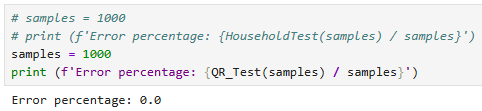
\includegraphics[scale=1]{./images/QRTest.png}
$$

\newpage
\bluebox{
\paragraph{Goal 2:} 
Using your $QR$ factorization, implement Algorithm 1. This is written as a matrix least squares problem, but think about the Frobenius norm and how you might be able to split it up into problems we know how to solve. \textbf{Please explain how you do this in the project report.} Practically, it is possible to then block some of these operations together for efficiency; you may take advantage of this if you wish.}
Given a QR factorization for $Z=QR$, and suppose $A-WZ^\top=B\in\mathbb R^{m\times n}$ 
\begin{align*}
  \norm{A-WZ^\top}_F^2&=\Tr \PAREN*{(A-WZ^\top)^\top (A-WZ^\top)}
  \\ &= \Tr \PAREN*{A^\top A} - 2\Tr \PAREN*{A^\top WZ^\top} + \Tr\PAREN*{ZW^\top WZ^\top}
\end{align*}

We wish to take the derivative with respect to $Z$. We observe the following:

\begin{align*}
  \nabla_W\Tr\PAREN*{A^\top A}&=0                      \\ 
  \nabla_W\Tr\PAREN*{2A^\top WZ^\top}&=-2AZ \\
  \nabla_W\Tr\PAREN*{ZW^\top WZ^\top}=\nabla_W\Tr\PAREN*{WZ^\top ZW^\top}&=2W Z^\top Z
\end{align*}

Setting the derivative to 0, we have:
\begin{align*}
  \nabla_Z\norm{A-WZ^\top}_F^2=0&=2WZ^\top Z-2AZ \\ 
  WZ^\top Z&= AZ \\
  Z^\top ZW^\top&=Z^\top A ^\top\\
  R^\top Q^\top QR W^\top&=R^\top Q^\top A^\top \\ 
  RW^\top&=Q^\top A^\top
\end{align*}

Thus, the $W$ that solves $RW^\top =Q^\top A^\top$ achieves the least squares minimum while holding $Z$ constant. Similarly, if we have a QR factorization $W=QR$, we have the least squares minimum while holding $W$ constant to be $RZ^\top=Q^\top A$. Since $R$ is upper triangular in both cases, we have an algorithm to solve for the argmin: use back substitution to solve the above systems for $W^\top$ and $Z^\top$. $Q^\top A$ can easily be calculated by applying the Householder vectors. Thus, we have the following algorithm:

\newpage 

\begin{algorithm}
  \caption{Alternating least squares, without regularization}
  \begin{algorithmic}[1]
    \State {\bf initialize} $W \in \R^{n_1 \times k}$, $Z \in \R^{n_2 \times k}$
      \While{not converged}
        \State $$Q_Z, R_Z \leftarrow (Z)$$
        \State $$Q_W, R_W \leftarrow (W)$$
        \State $$Z^\top \leftarrow R_W^{-1}Q_W^\top A$$ 
        \State $$W \leftarrow R_Z^{-1}Q_Z^\top A^\top$$ 
      \EndWhile
    \State {\bf return} $W$, $Z$
  \end{algorithmic}
\end{algorithm}

The Python implementation can be found in the appendix.\\

\bluebox{
\paragraph{Goal 3:}
Using your implementation, load the file Cornell.csv which has an image stored in the matrix $C$ and try to compute the best rank 75 approximation of the image. Compare this with the result of the best rank 75 image from the SVD (you can use a built in routine to compute this), what do you observe qualitatively and quantitatively?}



\newpage
\bluebox{
\paragraph{Question 1:}
Show that if we want to solve $$\min_x \|Ax-b\|_2^2 + \beta^2 \|x\|_2^2$$ we can instead solve 
\[
\min_x \left\|\begin{bmatrix}A \\ \beta I\end{bmatrix}x-\begin{bmatrix}b \\ 0\end{bmatrix}\right\|_2^2.
\]}

We observe the quantity that we want to minimize:
\begin{align*}
  \norm{Ax-b}_2^2+\beta^2\norm{x}_2^2 &= (Ax-b)^\top(Ax-b)+\beta^2x^\top x
  \\ &=x^\top A^\top Ax-b^\top Ax-x^\top A^\top b+b^\top b+\beta^2x^\top x
  \\ &=x^\top A^\top Ax+\beta^2 x^\top x - b^\top Ax - x^\top A^\top b+b^\top b
  \\ &= x^\top (A^\top A + \beta^2 I) x - (b^\top A + 0)x-x^\top (A^\top b + 0) + (b^\top b + 0)
  \\ &= x^\top \begin{bmatrix} A^\top & \beta I\end{bmatrix}\begin{bmatrix}A \\ \beta I\end{bmatrix} x - \begin{bmatrix}b^\top & 0\end{bmatrix}\begin{bmatrix}A \\ \beta I\end{bmatrix}x-x^\top \begin{bmatrix}A & \beta I\end{bmatrix} \begin{bmatrix}b \\ 0\end{bmatrix} + \begin{bmatrix}b^\top & 0\end{bmatrix}\begin{bmatrix}b \\ 0\end{bmatrix} 
  \\ &=\PAREN*{x^\top \begin{bmatrix} A^\top & \beta I\end{bmatrix} - \begin{bmatrix}b^\top & 0 \end{bmatrix}} \PAREN*{\begin{bmatrix} A \\ \beta I\end{bmatrix}x - \begin{bmatrix}b \\ 0 \end{bmatrix}}
  \\ &=\PAREN*{\begin{bmatrix} A \\ \beta I\end{bmatrix}x - \begin{bmatrix}b \\ 0 \end{bmatrix}}^\top \PAREN*{\begin{bmatrix} A \\ \beta I\end{bmatrix}x - \begin{bmatrix}b \\ 0 \end{bmatrix}}
  \\ &=\norm*{\begin{bmatrix} A \\ \beta I\end{bmatrix}x - \begin{bmatrix}b \\ 0\end{bmatrix}}^2_2
\end{align*}

Thus, since $\norm{Ax-b}_2^2+\beta^2\norm x_2^2=\norm*{\begin{bmatrix} A \\ \beta I\end{bmatrix}x - \begin{bmatrix}b \\ 0\end{bmatrix}}^2_2$, their minimums are the same, thus solving one is the same as solving the other problem.


\bluebox{
\paragraph{Goal 4:}
Using your $QR$ factorization, implement Algorithm 2. From the first set of goals, you should have worked out how to split this up into solving many least squares problems. Now, you have to think about what size those problems are, and which entries of the matrices they involve. Given that, you can then leverage your $QR$ factorization and the preceding item to implement the algorithm. \textbf{Please explain how you do this in the project report.}}

\newpage
\begin{algorithm}
\caption{Alternating least squares, with regularization and unknown entries}
\label{alg:als2}
\begin{algorithmic}[1]
\State {\bf initialize} $W \in \R^{n_1 \times k}$, $Z \in \R^{n_2 \times k}$
\While{not converged}
  \State $$Z \leftarrow \argmin_{Z}\left\|A - WZ^T\right\|^2_{F,\Omega} + \beta^2\left\|Z\right\|_F^2$$ 
  \State $$W \leftarrow \argmin_{W}\left\|A - WZ^T\right\|^2_{F,\Omega} + \beta^2\left\|W\right\|_F^2$$
\EndWhile
\State {\bf return} $W$, $Z$
\end{algorithmic}
\end{algorithm}

\bluebox{
\paragraph{Goal 5:}
Using your implementation, load each of the image files in Image*.csv and associated masks Mask*.csv, where * is 1, 2, and 3. Each file contains an image and the associated mask file contains an image of the same size whose entries are 1 if the corresponding entry of $C$ is observed and 0 if it is unobserved (so it defines the set $\Omega$). The unknown entries of $C$ have been set arbitrarily and you should not access or use them (as the will adversely affect your results). Using Algorithm~\ref{alg:als2}, try and recover each of the underlying images. You now have some parameters to consider and we encourage exploration of their values. You should not have to go to $k$ larger than 75 for any of the examples, and good $\beta$ to try are between $10^{-2}$ and 1. Report the images you recover, and discuss what you observe.}


\includepdf[pages=-]{./SVD-Image-Compression/code.pdf}

\end{document}
